\documentclass[11pt, a4paper]{article}
\usepackage{amsmath, amsthm, amssymb, calrsfs, wasysym, verbatim, bbm, color, graphics, geometry}
\usepackage[utf8]{inputenc} % comment when using lualatex
%\usepackage[italian]{babel} % lingua e a-capo-sillabato
\usepackage{fullpage}
\usepackage{graphicx}
%\usepackage[hidelinks]{hyperref,xcolor} % link di pagina
\usepackage[bottom]{footmisc} % note appiccicate al fondo della pagina
\usepackage{float} % per posizionamento immagini

\geometry{tmargin=.75in, bmargin=.75in, lmargin=.75in, rmargin = .75in}  

\newcommand{\R}{\mathbb{R}}
\newcommand{\C}{\mathbb{C}}
\newcommand{\Z}{\mathbb{Z}}
\newcommand{\N}{\mathbb{N}}
\newcommand{\Q}{\mathbb{Q}}
\newcommand{\M}{\mathbb{M}}
\newcommand{\Cdot}{\boldsymbol{\cdot}}

\newtheorem{thm}{Theorem}
\newtheorem{defn}{Definition}
\newtheorem{conv}{Convention}
\newtheorem{rem}{Remark}
\newtheorem{lem}{Lemma}
\newtheorem{cor}{Corollary}



\definecolor{dkgreen}{rgb}{0,0.6,0}
\definecolor{gray}{rgb}{0.5,0.5,0.5}
\definecolor{mauve}{rgb}{0.58,0,0.82}


\title{Latex Template }
\author{Raffaele Castagna}

\date{Academic Year 2025-2026}

\begin{document}

\maketitle
\tableofcontents
\newpage

\section{Intro to Cryptography}
\label{Intro}
\subsection{Secure Communication}
We have multiple goals in cryptography, the most important ones being:
\begin{center}
    \textbf{Confidential Integrity}
    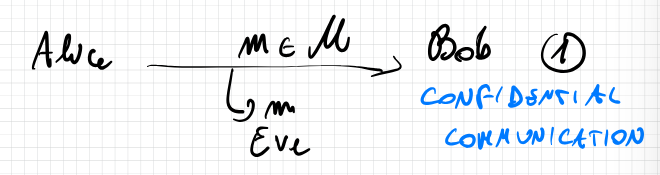
\includegraphics{img/CF comm.png}
\end{center}
\begin{center}
    \textbf{Message Integrity}
    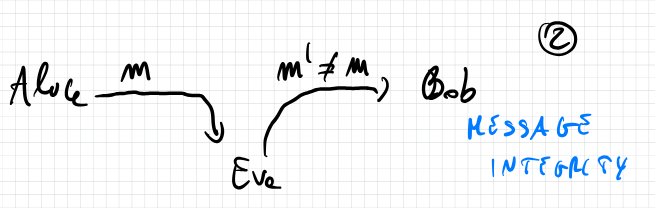
\includegraphics{img/Msg int.png}
\end{center}
Basically we want our message to be both \textbf{confidential}, so no-one except the intended target sees it and we it to be unmodified, so that its \textbf{integrity} has not been compromised.\\\\
There are many different ways to do this, but in our case we only see two major ways:
\begin{itemize}
    \item \textbf{Symmetric Cryptography}:  $\text{Where Alice and Bob share a key } k \in \mathcal{K} \text{,the key is random and unknown to Eve}$
    \item \textbf{Assymetric Cryptography}: Where Alice and Bob do not share a key, but they have each their own key pair $(p_k,s_k)$ where $p_k$ is the public key and $s_k$ is the secret/private key
\end{itemize}

\subsection{Unconditional Security}
To achieve confidential communication, we use symmetric cryptography.
\begin{center}
    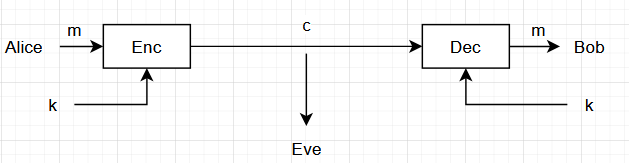
\includegraphics{img/US.png}
\end{center}
With $m \in \mathcal{M}, c \in \mathcal{C}, k \in \mathcal{K}$\\\\
In this case we have Alice sending a message \textit{m} which is then encrypted utilizing a randomly generate key \textit{k} to generate the cyphertext \textit{c}, after that to get back to the initial message \textit{m}, Bob will then need to decrypt it utilizing his own key \textit{k} on cyphertext \textit{c}.\\
In a more formal way we can define Symmetric encryption (SKE) as $\prod = (Enc, Dec)$ such that:
\begin{itemize}
    \item Enc : $\mathcal{M} \times \mathcal{K} \rightarrow \mathcal{C}$
    \item Dec: $\mathcal{C} \times \mathcal{K} \rightarrow \mathcal{C}$
    \item k is uniform over $\mathcal{K}$ (k is chosen according to some distribution)
\end{itemize}
An encryption scheme must satisfy the correctness requirement:
\begin{defn}
    $\forall k \in \mathcal{K}, \forall m \in \mathcal{M} \text{ it holds that } Dec(k,Enc(k,m)) = m$
\end{defn}

\textbf{Kerchoff's Principle}:
\begin{defn}
    Security should not depend on the secrecy of the algorithm but on the secrecy of the key.
\end{defn}
\subsection{Perfect Secrecy}
\begin{defn}
Let M be any distribution over $\mathcal{M}$ and K be uniform over $\mathcal{K}$ (Then observe C = Enc(K,M) in a distribution over C), we say that (Enc,Dec) = $\prod$ is \textbf{perfectly secret}
if $\forall M, \forall m \in \mathcal{M}, \forall c \in \mathcal{C}: Pr[M=m] = Pr(M=m | C=c)$ (The probability that M is m is equal to the probability that M is m knowing that C is c, so by knowing the cyphertext, we dont gain additional information).
\begin{lem}
The following are equivalent:
\begin{itemize}
    \item Perfect Secrecy
    \item M and C are independant
    \item $\forall m,m' \in \mathcal{M}, \forall c \in \mathcal{C}: Pr[Enc(k,m) = c] = Pr[Enc(k,m') = c] \text{ with k being uniform over } \mathcal{K}$
\end{itemize}
\end{lem}
\end{defn}
\subsection{OTP}
Let us see if OTP (\textit{One Time Pad}) is perfectly secret\\
We know that the OTP uses $\oplus$ to generate and later decypher the cyphertext, we have that $K=M=C=\{0,1\}^N$ with N being the length of the string, we know that:
\begin{itemize}
    \item Enc (k,m) = $k \oplus m$
    \item Dec (k,c) = $c \oplus k$ = $(k \oplus m) \oplus k = m$
\end{itemize}
To prove that it is perfectly secret let us utilize the third lemma:
\begin{center}
    $Pr[C=c | M=m'] = Pr[\text{Enc}_k (m') = c] = Pr[m' \oplus K = c] = Pr[K = m' \oplus c] = 2^{-N}$
\end{center}
and therefore:\\
\begin{center}
    $Pr[Enc(k,m') = c] = 2^{-N}$
\end{center}
There seem to be some limitations, the key can only be used once and it must as long as the message,lets assume we encrypt m'' and m':
$c_1 = k \oplus m_1\text{    } c_2 = k \oplus m_2 \text{ therefore } c_1 \oplus c_2 = m_1 \oplus m_2$, so if I know a pair $(m_1,c_1) \text{ then I could compute } m_2$, therefore we cannot encrypt two messages with the same key.
\begin{thm}
Let $\prod$ be a SKE then we have $|\mathcal{K}| \ge |\mathcal{M}|$.
\end{thm}
\begin{proof}
Take $\prod$ to be uniform over $\mathcal{M}$. Take any c s.t. Pr[C=c] $>$ 0.\\
Consider $\mathcal{M'} = \{Dec(k,c): k \in \mathcal{K}\}$ and assume $|\mathcal{K}| < |\mathcal{M}|$ by contraddiction, then:\\
\begin{center}
    $|\mathcal{M}|' \leq |\mathcal{K}| < |\mathcal{M}| \rightarrow |\mathcal{M'}| < |\mathcal{M}| \rightarrow \exists m \in \mathcal{M} \setminus \mathcal{M'}$
\end{center}
Now:\\
\begin{center}
    Pr[M=m] = $|\mathcal{M}|^{-1}$ but Pr[M=m | C=c] = 0
\end{center}

\end{proof}
\end{document}